\newpage

\setcounter{section}{5}
\section{Tests of Hypotheses}

You can generalize Neyman-Pearson Lemma to one-sided hypotheses tests, which will give a UMP (Uniformly Most Powerful) Test.

\setcounter{subsection}{5}
\subsection{GLR Test for Multinomial Distribution}
\graphicspath{{notes/img}}

\begin{enumerate}[a)]
    \item \textbf{Let $X_j$ be the count of dice rolls equal to $j$ (for $j \in \{ 1, \dots, 6 \}$) for $n$ iid rolls of a six-sided die. Use these to define the joint likelihood function $L(\theta_1, \dots, \theta_6)$ for the probabilities of the six faces $(\sum \theta_j = 1)$. Use Lagrange multipliers to show the MLE's are $\hat{\theta}_j = X_j / n,$ for $j \in \{ 1, \dots 6\}.$}  
    
     For $X_j$ the count of dice rolls equal to $j$ (for $j \in \{ 1, \dots, 6 \}$), the joint likelihood function for the $L(\theta_1, \dots, \theta_6)$ is
    \[
        L(\theta_1, \dots, \theta_6) = \frac{n!}{x_1! \dots x_6!}\theta_1^{x_1} \dots \theta_6^{x_6}.
    \]
    Equivalently, the log-likelihood is
    \[
        l(\theta_1, \dots, \theta_6) = \log \left(\frac{n!}{x_1! \dots x_6!}\right) + \sum_{i=1}^6 x_i \log(\theta_i)
    \]
    where $\sum \theta_i = 1$. \\

    To determine the MLE's $\hat{\theta}_i$, we use Lagrange Multipliers and work to maximize
    \[
        l(\theta_1, \dots, \theta_6, \lambda) = \log \left(\frac{n!}{x_1! \dots x_6!}\right) + \sum_{i=1}^6 x_i \log(\theta_i) + \lambda\left(\sum_{i=1}^6 \theta_i - 1\right)
    \]
    where the extra $\lambda(\sum\limits_{i=1}^6 \theta_i - 1)$ term comes from the Lagrange multiplier $\lambda$ and the constraint $\sum \theta_i = 1$. \\
    
    To maximize $l(\theta_1, \dots, \theta_6, \lambda)$, we need the partials with respect
    to each $\theta_i$ and $\lambda$ to be equal to $0$:
    \[
        \frac{\partial l}{\partial \theta_i} = \frac{x_i}{\theta_i} + \lambda = 0 \text{ and } \frac{\partial l}{\partial \lambda} = \left(\sum \theta_i \right) - 1 = 0.
    \]
    The former condition $\frac{x_i}{\theta_i} + \lambda = 0$ tells us that $\hat{\theta}_i = -\frac{x_i}{\lambda}$. \\
    
    Now, the latter condition $\left(\sum \theta_i \right) - 1 = 0$ tells us that
    \[
        \sum \hat{\theta}_i = - \frac{\sum x_i}{\lambda} = 1,
    \]
    and solving for $\lambda$ gives us $\hat{\lambda} = - \sum x_i$. Thus, for each $\hat{\theta}_i$, we know that
    \[
        \hat{\theta}_i = -\frac{x_i}{\lambda} = \frac{-x_i}{- \sum x_i} = \frac{x_i}{n}
    \]    
    as desired. 

    \newpage
    
    \item \textbf{Derive the GLR test of $H_0 \colon \theta_1 = \dots = \theta_6$ vs $H_1 \colon$ not $H_0$. Suppose $n=24$ rolls gave counts of $X_1 = 8$, $X_2 = X_3 = X_4 = X_5 = 4$, and $X_6 =0$. Show how simulation may be used to compute an exact $p$-value. Compare to using the Chi-square approximation for $-2\log \Lambda$.} 
    
    As we saw previously, 
    \[
        L(\theta_1, \dots, \theta_6) = \frac{n!}{x_1! \dots x_6!}\theta_1^{x_1} \dots \theta_6^{x_6}
    \]
    Our null hypothesis is $H_0\colon \theta_1 = \dots = \theta_6 = \frac{1}{6}$ and alternative hypothesis is $H_1\colon$ not $H_0$, so
    \begin{align*}
        \Lambda &= \frac{\max\limits_{H_0} \frac{n!}{x_1! \dots x_6!}\theta_1^{x_1} \dots \theta_6^{x_6}}{\max\limits_{H_0 \cup H_1} \frac{n!}{x_1! \dots x_6!}\theta_1^{x_1} \dots \theta_6^{x_6}} \\
        &= \frac{\left( \frac{1}{6} \right)^{x_1 + \dots + x_6} }{\left( \frac{x_1}{n} \right)^{x_1} \dots \left( \frac{x_6}{n} \right)^{x_6} }
    \end{align*}
    where the denominator is from the fact that $\hat{\theta}_i = \frac{x_i}{n}$, which we derived in part (a). Note that
    \begin{align*}
        -2 \log (\Lambda) &= -2 \sum_{i=1}^6 x_i \log \left( \frac{\frac{1}{6}}{\frac{x_i}{n}} \right) \\
        &= -2 \left( \sum x_i \log \frac{1}{6} - \sum x_i \log \left( \frac{x_i}{n} \right) \right) \\
        &= -2 \left( n \log \left(\frac{1}{6}\right) - \sum \log \left( \left( \frac{x_i}{n} \right)^{x_i} \right) \right) 
    \end{align*}

    The Chi-square approximation for $-2 \log \Lambda \, \dot\sim \, \chi^2_{\nu}$ where $\nu$ is the difference in the dimensions of the null and alternative parameter spaces; in this case, $\nu = 6 - 1 = 5$. \\

    For the given data, we find that 
    \[
        \Lambda = \frac{\left( \frac{1}{6} \right)^{24} }{\left(\frac{8}{24}\right)^8 \left(\frac{4}{24}\right)^{16}} = \frac{1}{256}
    \]
    so $-2 \log \Lambda \approx 11.1$. Using the Chi-Square approximation $\chi^2_5$, we find the associated p-value using the R command \textit{$1$ - pchisq($11.1, 5)$ = 0.049}.
    We can compare this approximation to the exact p-value which we can acquire through simulation (see attached R Code). \\

    Note that the interpretation of the p-value is the probability of achieving such an extreme value of $-2\log \Lambda$ in $n$ rolls, assuming $H_0$ is true. 

    \newpage
    
    \item \textbf{For a $2$-way table of counts, derive the GLR test for independence of the row and column variables. Show that the Chi-square approximation for $-2 \log \Lambda$ is asymptotically equivalent to the Pearson Chi-square test of independence (See Rice 9.5, 13.4).}
    
     See the image below for the GLR test for independence of the row and column variables in a two-way table of counts.\\
    
    \begin{center}
    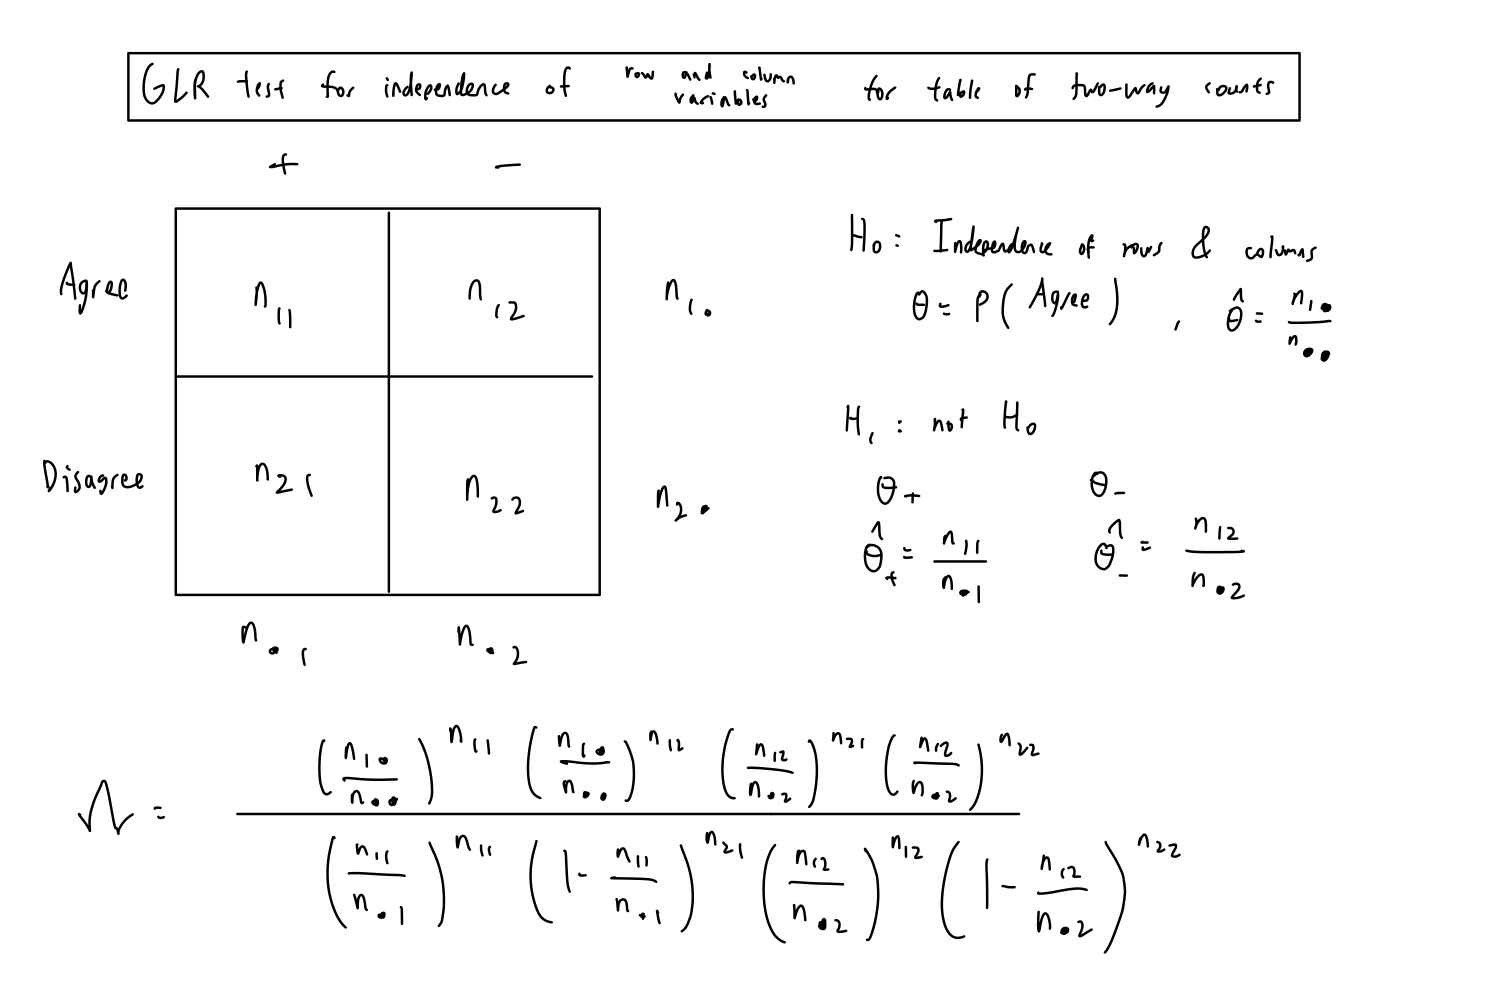
\includegraphics[scale=0.25]{week6_c.jpeg}
    \end{center}

    To show the asymptotic equivalence of the Chi-square approximation for $-2 \log \Lambda$ with the Pearson Chi-square test of independence, we will manipulate the expression for $-2 \log \Lambda$. \\
    
    Note that 
    \[
        \Lambda = \prod_{i=1}^{2}\prod_{j=1}^2 \frac{\theta_{ij}^{x_{ij}}}{\hat{\theta}_{ij}^{x_{ij}}} = \prod_{i=1}^{2}\prod_{j=1}^2 \left( \frac{\theta_{ij}}{\hat{\theta}_{ij}}\right)^{x_{ij}}.
    \]
    It follows that
    \begin{align*}
        -2 \log \Lambda &= 2 \sum_{i=1}^{2} \sum_{j=1}^2 x_{ij} \log \left( \frac{\hat{\theta}_{ij}}{\theta_{ij}} \right) \\
        &= 2n \sum_{i=1}^{2} \sum_{j=1}^2 \hat{\theta}_{ij} \log \left( \frac{\hat{\theta}_{ij}}{\theta_{ij}} \right)
    \end{align*}
    where the second step follows from the fact that $x_i = n\hat{\theta}_{ij}$. \\

    Note furthermore that for large $n$, we should expect $\hat{\theta}_{ij} \approx \theta_{ij}$. Since the Taylor Series expansion of the function
    \[
        f(x) = x \log \left( \frac{x}{x_0} \right)
    \] 
    about $x_0$ is $f(x) = (x - x_0) + \frac{1}{2} (x-x_0)^2 \frac{1}{x_0} + \dots,$ we find that
    \begin{align*}
        -2 \log \Lambda &= 2n \sum_{i=1}^{2} \sum_{j=1}^2 \hat{\theta}_{ij} \log \left( \frac{\hat{\theta}_{ij}}{\theta_{ij}} \right) \\
        &\approx 2n  \left[\sum_{i=1}^{2} \sum_{j=1}^2 \left( \hat{\theta}_{ij} - \theta_{ij} \right) +  \frac{1}{2} \frac{(\hat{\theta}_{ij} - \theta_{ij})^2}{\hat{\theta}_{ij}}\right] \\
        &\approx 2n  \sum_{i=1}^{2} \sum_{j=1}^2 \left( \hat{\theta}_{ij} - \theta_{ij} \right) + n \sum_{i=1}^2 \sum_{j=1}^2 \frac{(\hat{\theta}_{ij} - \theta_{ij})^2}{\hat{\theta}_{ij}}
    \end{align*}

    Note that by definition, 
    \[
        \sum_{i=1}^{2} \sum_{j=1}^2 \hat{\theta}_{ij} = \sum_{i=1}^{2} \sum_{j=1}^2 \theta_{ij} = 1
    \]
    so the first term in the approximation is $0$. Thus, we find that
    \begin{align*}
        -2 \log \Lambda &\approx n \sum_{i=1}^2 \sum_{j=1}^2 \frac{(\hat{\theta}_{ij} - \theta_{ij})^2}{\hat{\theta}_{ij}}\\
        &\approx \sum_{i=1}^2 \sum_{j=1}^2 \frac{(n\hat{\theta}_{ij} - n\theta_{ij})^2}{n\hat{\theta}_{ij}} \\
        &\approx \sum_{i=1}^2 \sum_{j=1}^2 \frac{(x_{ij} - n\theta_{ij})^2}{n\hat{\theta}_{ij}}
    \end{align*}
    where once again the final step follows from the fact that $x_{ij} = n\hat{\theta}_{ij}$. \\
    
    This is simply the test statistic for the Pearson Chi-Square test for independence, so
    we conclude that the Chi-square approximation for $-2\log \Lambda$ is asymptotically equivalent to the Pearson Chi-square test of independence, as desired.
    
    
\end{enumerate}
